\chapter{Perihperals}
Peripherals in our context can have two meanings. Either, they could be the devices around the microcontroller on the development board like the LCD, push-buttons, potentiometers, temperature sensor or EEPROM which the microcontroller is able to interact with, usually for the purpose of getting input, displaying output or storing data. Alternatively, peripherals could refer to the blocks of circuitry inside of the microcontroller which provides some additional functionality which the CPU does not have. Examples would include circuitry for providing precise timing, or circuitry to interact with the pins of the microcontroller. To distinguish between the two, we call those peripherals which are outside of the microcontroller development board peripherals, and those which are inside the microcontroller chip we call internal peripherals. 

The general structure is that the CPU interfaces with internal peripherals which in turn interface with dev board peripherals through the pins on the microcontroller.

\section{Internal Peripherals}
All internal peripherals are organised in a bus architecture which allows the CPU to interact with them. The full diagram of all of the peripherals in the STM32F051 is shown on the following page.
\afterpage{
  \centering
  \includepdf[pages={11}]{./STM32F051_datasheet.pdf}
}
In order for the CPU to interface with them, each peripheral has a block of memory associated with it. Recall the address space of the microcontroller as shown in \autoref{fig:memory_map}. The block called \emph{peripherals} running from address 0x4000 0000 to 0x4800 17FF is the range of addresses which is available to have peripherals associated with it. The full memory map can be seen in Figure 2 of the Reference Manual. 

Out of that large peripherals block of memory, each peripheral has a specific block of memory associated with it. The starting and ending address for each peripheral in the microcontroller can be seen in Table 1 of the Reference Manual. Note how the vast majority of the peripherals address space is unimplemented (or "reserved"). This allows there to be lots of space for expansion: fancier micrcontrollers can have more peripherals and make use of this unimplemented address space. 

Inside each block of memory assigned to a specific peripheral is further sub-divisions of the block into \emph{registers}. Registers are blocks of memory (typically one word big on our processor) which provide a specific, well defined element of functionality, typically configuring how the peripherals works or providing some status information about the peripheral. The CPU is able to write data to a register to configure the peripheral or read data from a register to get information about the peripheral. Sometimes a register simply holds a number (for example: for use in a counter) but more frequently each individual bit in a register as a specific meaning. For example, a bit can be set high to enable some sort of functionality or set low to disable some functionality. 

Each register has an address which must be known when interacting with that register. The way that the address is calculated is using a (base address) plus (offset) system. The base address is the start of the address range for the peripheral as seen in Table 1 of the Reference Manual, and the offset is the number which must be address to the base address to get the effective address of the register. This is a very convenient system as our load and store operations in the CPU also work on a base plus offset system. 

A description of what each register does (and indeed what each bit in the register does) as well as the offset for that specific register can be found at the end of the chapter of the Reference Manual which deals with the peripheral (or class of peripherals) which you're trying to interact with. 

A register is like RAM in that it is volatile memory, but it is different to RAM in that while RAM is general purpose memory which can be used for storing whatever you like, each register has a specific function and very specific, meaningful data must be written to or read from the peripheral which will configure the microcontroller in some way.

The following chapters serve to describe the operation of some of the key peripherals in the microcontroller.

